\documentclass[a4paper,12pt]{scrartcl}
\usepackage{libertine}

\usepackage[\directlua{if os.getenv("USER")=="john" then tex.sprint([=[ EU2 ]=]) else tex.sprint([=[T1]=]) end} ]{fontenc}
%\usepackage[EU2]{fontenc}
%\usepackage[T1]{fontenc}
\usepackage[utf8]{luainputenc}
\usepackage{graphicx}
\usepackage{luatextra}
%\usepackage{ngerman}
%\usepackage[ngerman]{babel}
%\usepackage{babelbib}
\usepackage{listings}
\usepackage{color}
\usepackage{url}
\usepackage{bytefield}
%TIKZ--------------------------------------
\usepackage{tikz}
\usetikzlibrary{positioning}
\usetikzlibrary{fit}
\pgfdeclarelayer{background}
\pgfdeclarelayer{belowmain}
\pgfdeclarelayer{foreground}
\pgfsetlayers{background,belowmain,main,foreground}
%------------------------------------------

\newcommand{\haqbus}{ha\textsuperscript{q}\textsubscript{b}us}


\usepackage[pdftex=true,colorlinks=true,linkcolor=black,urlcolor=blue,citecolor=black]{hyperref} 
\title{\haqbus}
\author{C3D2}


\date{}
\makeindex

\definecolor{listinggray}{gray}{0.94}

%anschalten um trennstellen zu sehen:

%\directlua{ show_hyph = function(head) while head do if head.id == 0 or head.id == 1 then show_hyph(head.list) elseif head.id == 7 then local n = node.new("whatsit","pdf_literal") n.mode = 0 n.data = "q 0.3 w 0 2 m 0 7 l S Q" n.next = head.next n.prev = head head.next = n head = n end head = head.next end return true end luatexbase.add_to_callback("post_linebreak_filter",show_hyph,"show_hyph") } 


\begin{document}
\maketitle

\begin{abstract}
This is the very first draft of the \haqbus protocol specification. The haqbus is an EIA-485 (aka RS-485) based field communication system connecting arbitrary devices for hackerspace-automation.
\end{abstract}

\vspace{5cm}
\thispagestyle{empty}
\begin{center}
from Dresden with love by \\
\Large
< < < / > >  \\
\Large
Chaos Computer Club Dresden, c3d2.de \\
\biolinumGlyph{Tux} timestamp: \directlua{tex.print(os.time())}  \biolinumGlyph{Tux}
\end{center}
test hier: \directlua{if os.getenv("USER")=="john" then tex.sprint([=[ EU2 ]=]) else tex.sprint([=[T1]=]) end} ende 
\newpage
\tableofcontents
\newpage
%===============================================================
\section{Introduction}
Standards are cool, everybody should have some and stick to them!

%Each computer sciene professional should at least once in his live design a communication protocoll to understand lon what a fragile little world we are living.

\section{Usecases, Features, and Requirements}

In case of a collision on the bus, that is, two devices are sending data at the same time, we either receive:
\begin{itemize}
\item nothing,
\item garbage, or
\item correct data, in case two devices are sending identical data and we have good conditions for (un)lucky coincidences.
\end{itemize}
Therefore we cannot make any assumption on what will happen in this case.

\begin{itemize}
\item up to about 200 devices per bus segment
\item fast auto discovery and negotiation of devices
\item collision avoidance
\item no realtime guarantees yet, as-fast-as-possible communications
\item single busmaster, multiple busmaster capable candidates
\item busmaster handover to other busmaster capable devices

\end{itemize}



\section{Architectural Overview}
\subsection{Participants and their Roles in haqbus}
There ar two kinds of devices partaking in comunication: Those who are capable of becoming busmaster and those who aren't.
The first are called \emph{potential busmaster} or PBM, the latter \emph{not master capaple} or NMC.
As a matter of fact, there is no problem in designing all devices as PBMs, for practical reasons this might not be desired as it will
slow down busmaster negotiation and cost resources wich can be scarce on small devices. 
There must be at least one PBM on each bus segment.
Each device has a firmware or hardware defined globally unique hardware identifier, similar to a MAC address.
Whether this MAC is 2, 4, or 8 byte long is still 

There are currently 4 roles in which a device could participate in a \haqbus installation:
\begin{enumerate}
\item active busmaster (ABM)
\item standby, or sleeping, busmaster (SBM)
\item passive slave (PAS)
\item not attached (NOA) 
\end{enumerate}

\begin{table}
  \centering
    \begin{tabular}{|l|l|}
        \hline
        device type & device role \\ \hline
        PBM         & ABM         \\ 
        PBM         & SBM         \\ 
        PBM         & NOA         \\
        NMC         & NOA     \\
        NMC         & PAS         \\
        	 
        \hline
    \end{tabular}
    \caption{%
    All valid combinations of device types and their roles.    
    }
\end{table}

Keep in mind, that a SBM is a PBM-device, that in most cases acts very much like an NMC-device in its role as PAS, with the one difference,
that it can become an ABM if required, e.g. if there is no other ABM on the bus.
A PBM- or NMC-device will change its role to NOA when powered on and further change its role to SBM, or PAS when it is recognized by the ABM.
In case there is no ABM present, a PBM in NOA-role will become the new ABM.

If you understood the last paragraph, you will have memorized by now the shorthands for devices and their roles -- which is a
good thing as you will definitly need them in the following sections.

\subsection{Basic Interaction between Participants}
Rule 1: The active busmaster is responsible for doin' all the stuff. (At least mostly all off the time.)

The thing we want to do is, to avoide all possible collisions by using time division multiple access
(TDMA) with dynamic timeslots that are coordinated by the ABM.

\begin{itemize}
\item If an ABM is present, it is the only device that is allowed to speak without permission.
\item The ABM tells other devices (SBM, PAS, and NOA) in regular intervalls when and for how long they are allowed to speak.
\item The ABM respect these time periods and doesn't interfere while a SBM, a PAS or a NOA is speaking.
\item SBM and PAS speak only when they are asked to and no longer than they are allowed.
\item NOA speak only, when asked by the ABM (discovery) or when they detect that there is no ABM present (master discovery).
\end{itemize}

Once, an ABM is established and in control, this should provide a reasonable stable and deterministic flow of data without any collision.
Whether this is still the case in situations where data packets get corrupted is still to examine!
However, this can only be applied after a discovery phase, which will be discussed in section FIXME.

\subsection{Operational Status of the Bus}
The bus as a whole system hast only three status\footnote{Yes, AFAIK this really is the plural of status, it's pronounced with a long `u'.}:
\begin{itemize}
 \item CHAOS is the state after power on. There is no ABM present and all devices are NOA. Master discovery happens to end CHAOS and achieve PENTA.
 \item PENTA is the normal and well ordered operational state. It is achieved after a master discovery led to the negotation of one single ABM.
 \item B0RKEN happens sometimes when an ABM drops out without handing over the ABM role to another PBM, e.g. when just switchig off the ABM.
\end{itemize}
B0RKEN can be treated the same way as CHAOS, but there might be a slightly more elegant solution as all the remaining SBMs should know of each others existence.
After master discovery during CHAOS, there is no dedicated discovery phase, as discovery happens all the time and is interwoven with normal operation during PENTA.



\section{Layer Specification}
Bus communication is done in 4 different Layers ... or 3 or 5 or 23?? FIXME
They correspond to the famous ISO/OSI layer model as follows... NOT , so FIXME

%Traditional OSI ISO Stuff:
%Layer 1: physical layer	PLEASE
%Layer 2: data link layer	DO
%Layer 3: network layer		NOT
%Layer 4: transport layer	THROW
%Layer 5: session layer		SALAMI
%Layer 6: presentation layer	PIZZA
%Layer 7: application layer	AWAY
%Layer 8: user

\subsection{Layer one (nameme osi 1)}
There is only on main channel and the symbol rate of the main channel is to be 500.000 baud. 
The main channel is provided by a two wire TIA/EIA-485 \cite{EIA485} bus, also known as RS485.


\subsubsection{Cable Definition}
The used cables are twisted pair cables of 4 pairs plus shielding, that are commonly used for PentanewsGameshow buzzers
or more arcane installations like Ethernet cabeling.
The standard suggested is EIA/TIA-568A~\cite{EIA568}. But if rule No. 1 of RFC1925 \cite{RFC1925} is adhered to, everything else will be fine.

\begin{table}
	\centering
	\begin{tabular}{l c l}
		number        & sugested color      & usage \\
		\hline
		1             & white/green stripe  &   GND \\
		2             & green solid         &   GND \\
		3             & white/orange stripe &   signal RS485-A\\
		4             & blue solid          &   VCC \\
		5             & white/blue stripe   &   VCC \\
		6             & orange solid        &   signal RS485-B\\
		7             & white/brown stripe  &   spare signal C \\
		8             & brown solid         &   spare signal D \\
	\end{tabular}
	\caption{%
	Overview of wire asignment  \newline%
	Numbers correspond to pin numbers of an RJ-45 connector as shown in figure~\ref{fig:rj45}.
	}
	\label{tab:wires}
\end{table}

\begin{figure}
	\centering
	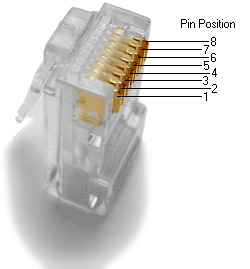
\includegraphics[scale=.7]{png/Rj45plug-8p8c.png}
	\caption{wire numbering on rj45 connector}
	\label{fig:rj45}
\end{figure}

\subsection{Layer two (nameme osi 2+3)}

\subsubsection{Busmaster Discovery and Negotiation}
At cold start or when the current busmaster drops out (disconnected, failure), there will be no communication flow on the bus.
When this is detected, the busmaster role must be negotiated between all busmaster capable device.

TODO: Describe busmaster discovery and negotiation.


FIXME: Should there be an announcement of the protocol version in use?
This way an upgrade to more advanced future protocols (e.g. real time capable with timeslots) will be easier.


\subsubsection{Bus Checking Phase}
During the bus checking phase the busmaster checks which of all registered devices are still alive. For this the busmaster iterates over its internal table of registered devices and sends a paket of type ASKSTAT~\ref{cp:ASKSTAT} to them.

\subsubsection{Paket Types}
All Pakets of this layer are at least 4 Bytes long and prefixed with the packet delimiter Byte 0x00. 
Since 0x00 is the paket delimiter any 0 Byte in all other fields of a packet  must be escaped
% FIXME - uuuhh, thats not good. Maybe there is a more elegant solution....

\paragraph{ASKSTAT}

ABM asks a SBM or PAS for status
\label{cp:ASKSTAT}
\begin{figure}[h!]
\begin{bytefield}{32}
\bitheader{0,7,8,15,16,23,24,31} \\
\small
\bitbox{8}{\mbox{<ASKSTAT>}}&\bitbox{8}{check8}&\bitbox{16}{Addr:Reciver}
\end{bytefield}
\end{figure}

\paragraph{STALIVE}
Normal status answer. SBM or PAS sends this, to acknowledge an ASKSTAT when they have nothing to say.
\label{cp:STALIVE}
\begin{figure}[h!]
\begin{bytefield}{32}
\bitheader{0,7,8,15,16,23,24,31} \\
\small
\bitbox{8}{<STALIVE>}&\bitbox{8}{check8}&\bitbox{16}{Addr:Reciver}
\end{bytefield}
\end{figure}


\paragraph{STALIVPL}
This is similar to STALIVE, but a short payload data sequence to arbitrary devices that have an address (all except NOA) is included.
\label{cp:STALIVPL}
\begin{figure}[h!]
\begin{bytefield}{32}
\bitheader{0,7,8,15,16,23,24,31} \\
\small
\bitbox{8}{<STALIVPL>}&\bitbox{8}{check8}&\bitbox{16}{Addr:Reciver}\\
\wordbox{3}{Payload}\\
\end{bytefield}
%Where the Payload is up to 28 bytes of the form:
%\begin{bytefield}{32}
%\bitbox{8}{len}&\bitbox{24}{data\ldots} \\
 %\bitbox{16 CRC16}\\
%\end{bytefield}
\end{figure}
%FIXME how is the length of payöoad determined?
The maximum length of a STALIVEPL-Packet is still to be negotiated but probably 32 byte.
% 



\paragraph{ASKSTATXXX}  Is for the transmisson of p0rn packets only.
\label{cp:ASKSTATXXX}
\begin{figure}[h!]
\begin{bytefield}{32}
\bitheader{0,7,8,15,16,23,24,31} \\
\small
\bitbox{8}{Type:ASKSTAT}&\bitbox{8}{check8}&\bitbox{16}{Addr:Reciver}
\end{bytefield}
\end{figure}



\section{More Layers}
TODO: specify me!

\newpage
\bibliographystyle{gerplainurl}
%\nocite{LINUX}
\bibliography{spec} 

\end{document}

